\documentclass[12pt, letterpaper]{article}

%Line Spacing
\usepackage{setspace}
\doublespacing

%Graphics
\usepackage{graphicx}

%Margins
\usepackage[margin=1in]{geometry}

%Citations
\usepackage[backend=biber,style=ieee,urldate=long]{biblatex}
\addbibresource{refs.bib}

\title{Passwordless Authentication}
\author{Zachary Thompson}

\begin{document}
\maketitle

\section{Executive Summary}
\section{Introduction}
Passwordless authentication describes a collection of authentication methods which do not rely on the user remembering and entering a password in order to be authenticated.
Proponents of passwordless authentication argue it is both more convenient and more secure than traditional, password-based authentication.

This paper will look at the flaws of password based authentication and analyze whether passwordless authentication can address them.
It will describe various methods of passwordless authentication and discuss their benefits and drawbacks.
\section{Discussion}
\subsection{The Problem With Passwords}
Password-based authentication has a number of flaws.
For one, passwords are prone to reuse.
It is difficult to remember dozens of unique passwords, so people end up using the one they already memorized over and over again.
According to a poll conducted by Google and Harris in 2019, 52\% of people reuse a password for multiple accounts and 13\% reused a password for all of their accounts \parencite{googleharris2019poll}.
If an attacker were to compromise one password, then there is a good chance they could use it to breach other accounts.

Another problem is that good passwords are difficult to memorize.
Good passwords are long and use different types of symbols.
Ideally, a password would be a long, randomly generated string of characters.
A password like that is hard enough to memorize for one website, let alone all of them.

Password managers help in this regard.
They are able to generate and store passwords for you.
This means that, assuming the password manager is used correctly, all of your passwords will be difficult to crack and will be unique. 
However, all of your passwords are now only as strong as your master password (and the security of your password manager).

%Password managers dont address phishing and may be more succeptable due to autofill

\subsection{A Solution: Get Rid of the Password}
Perhaps one way to eliminate the problems of passwords is to use some other form of authentication.
That is exactly what Microsoft allows you to do with their Authenticator app. 

\begin{figure}[h]
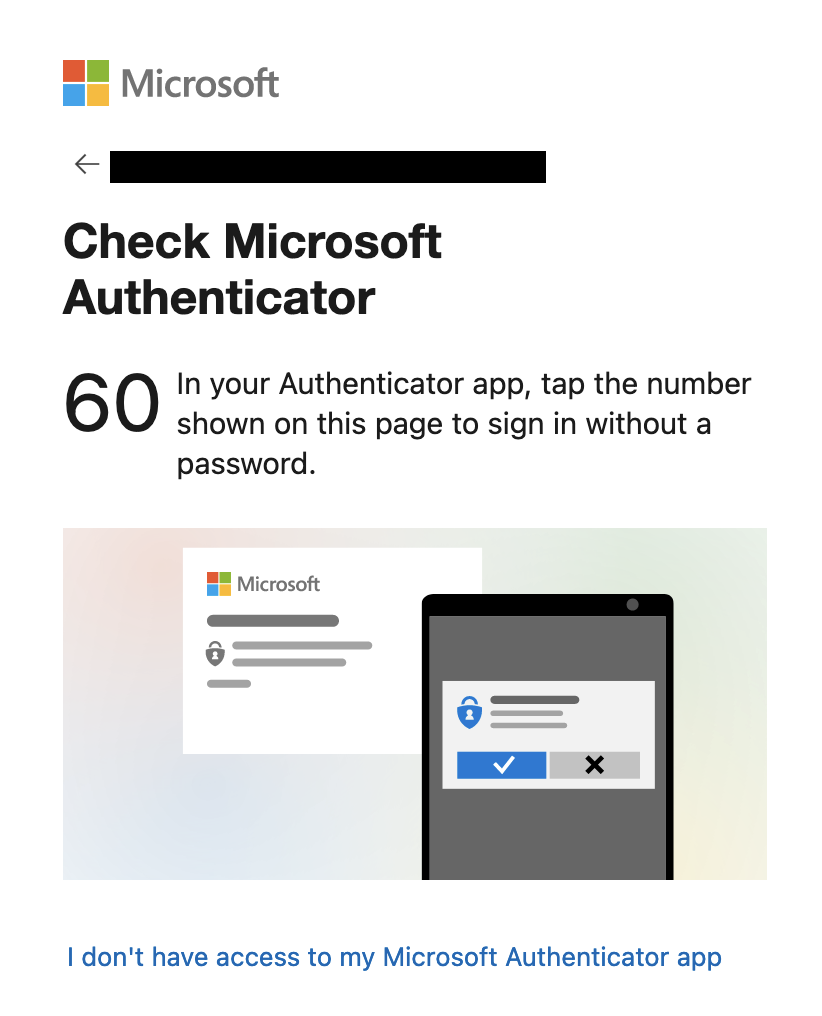
\includegraphics[width=0.5\textwidth]{mslogin.png}
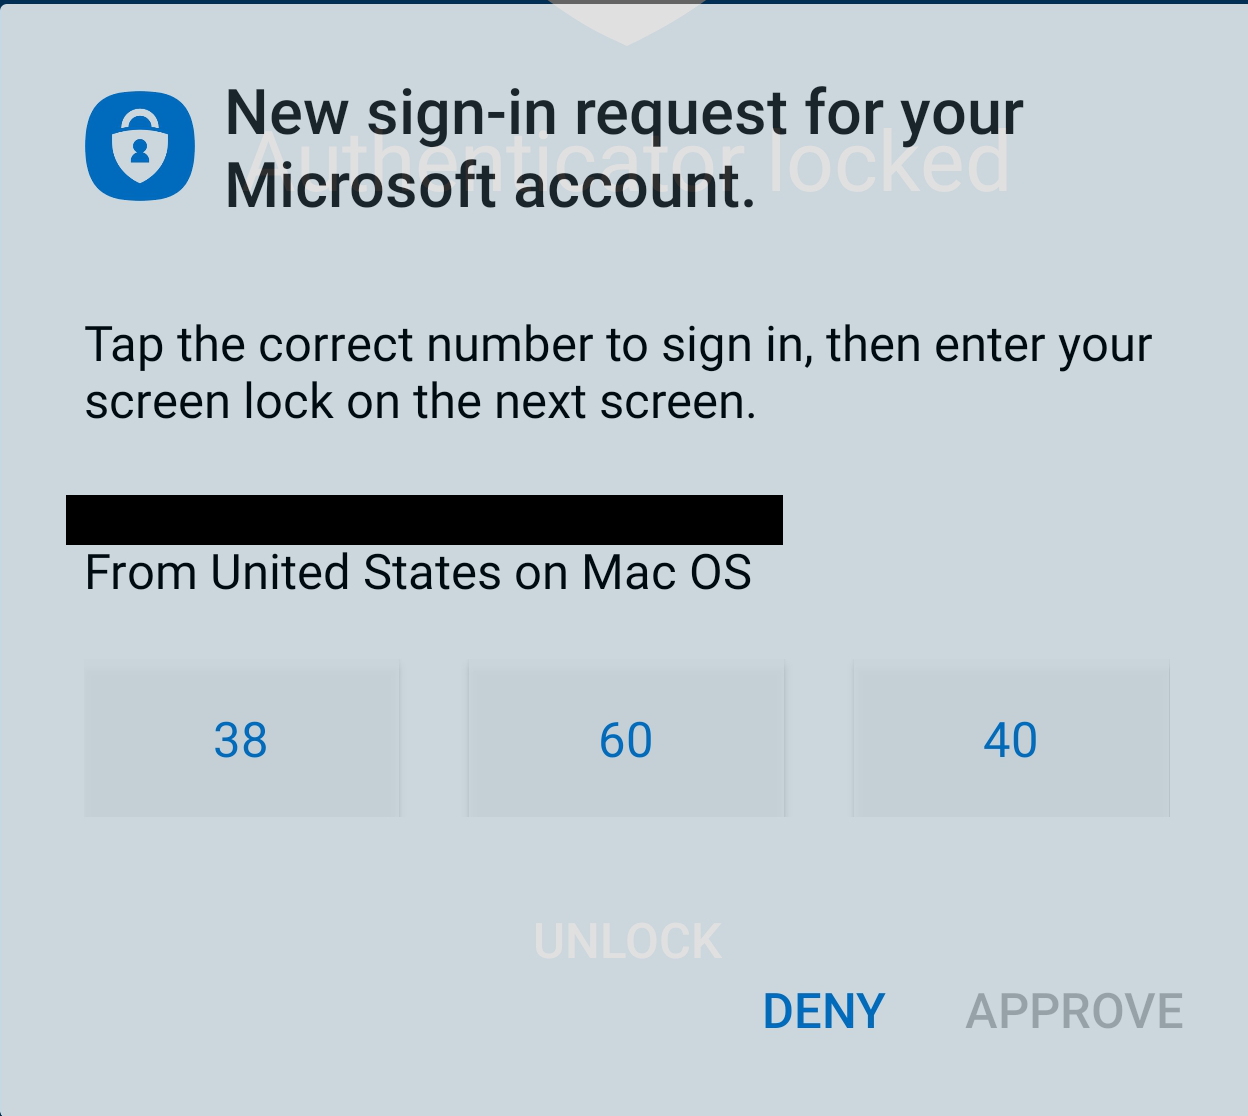
\includegraphics[width=0.5\textwidth]{authenticator.png}
\caption{Blah blah blah\label{msauth}}
\end{figure}

\subsection{Account Recovery}
If the user is no longer able to access their authentication method, then there needs to be some form of account recovery so that the user can fix the issue.

\section{Analysis and Recommendations}
\section{Conclusion}

\printbibliography
\end{document}
